\chapter{Il PROLOG}

\dfn{PROLOG}{
  PROLOG (Programming Logic) è un \newfancyglitter{linguaggio dichiarativo} basato sul \newfancyglitter{paradigma logico}: 
  \begin{itemize}
    \item Non si descrive cosa fare per risolvere un problema. 
    \item Si descrive la situazione reale con \newfancyglitter{fatti} e \newfancyglitter{regole} e si chiede all'interprete di verificare se un \newfancyglitter{goal} segue oppure no secondo una logica classica.
  \end{itemize}
}

\nt{Il PROLOG è equivalente alla logica dei predicati del primordine.}

\section{Le Basi}

\dfn{Fatti}{Si rappresenta con dei \newfancyglitter{fatti} un dominio di interesse.}

\ex{Fatto}{
  Fatto per descrivere che un alimento contiene più calorie di un altro: 
  \begin{itemize}
    \item piuCalorico(wurstel, banana). 
    \item Rappresenta il fatto che il würstel è un alimento maggiormente
calorico rispetto alla banana.
  \end{itemize}
}

\dfn{Regole}{
  Si rappresentano le possibili inferenze con delle \newfancyglitter{regole}: 
  \begin{center}
    \texttt{head := subgoal1, subgoal2, \dots, subgoaln}
  \end{center}
}

\ex{Regola}{
  \begin{center}
    \texttt{felino(X) := gatto(X)}
  \end{center}
  Rappresenta la regola che permette di concludere che i gatti sono felini.
}

\paragraph{Idee di base del PROLOG:}

\begin{itemize}
  \item Regole ricorsive.
  \item L'interprete analizza i fatti e le regole nell'ordine in cui si trovano nel programma. 
  \item Meccanismo di pattern matching per uni care
variabili e termini. 
\item L’interprete, dato un programma, cerca di
dimostrare un goal considerando fatti e applicando
regole, nel secondo caso generando sotto-goal.
\end{itemize}

\dfn{Clausole}{
  Le clausole sono i fatti o le regole. Contengono:
  \begin{itemize}
    \item Atomi: 
      \begin{itemize}
        \item Costanti. 
        \item Numeri.
      \end{itemize}
    \item Variabili.
    \item Termini Composti, ottenuti applicando funtori a termini.

  \end{itemize}
}

\nt{Un programma PROLOG è un insieme di clausole.}

\clm{}{}{
  \begin{itemize}
    \item L'estensione dei file PROLOG è 'pl'.
    \item In PROLOG le variabili hanno l'iniziale maiuscola. 
    \item L'unica struttura dati nativa è la lista.
    \item Per eseguire swi: swipl. 
    \item Per compilare: $[$'nomefile.pl'$]$.
    \item Il comando ';' indica possibili alternative.
    \item Il comando 'trace.' consente un esecuzione passo per passo.
    \item '\textbackslash +' rappresenta la negazione per fallimento. 
    \item L'ordine è importante perché PROLOG "legge" dall'alto verso il basso.
\end{itemize}
}

\paragraph{Qualche predicato \fancyglitter{built-in}:}

\begin{itemize}
  \item \texttt{var(X)}: indica se \texttt{X} è una variabile. 
\item \texttt{ground(X)}: indica se \texttt{X} è istanziata. 
\item \texttt{atom(X)}: indica se \texttt{X} è atomica. 
\end{itemize}

\subsection{Liste}

\dfn{Lista}{
  La \newfancyglitter{lista} è la struttura dati principale in PROLOG. Una lista è caratterizzata da una testa e da una
coda: 
\begin{itemize}
  \item Testa: primo termine (a sinistra) della lista. 
  \item Coda: la lista dei termini dal secondo (incluso)
in poi.
\end{itemize}
}

\nt{Rappresentata come $[$Head $|$ Tail$]$.}

\begin{figure}[h]
    \centering
    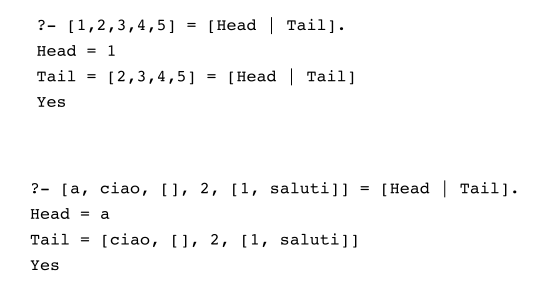
\includegraphics[scale=0.6]{01/liste.png}
    \caption{Le liste in PROLOG.}
\end{figure}

\paragraph{Predicati \fancyglitter{built-in}:}

\begin{itemize}
  \item \texttt{length(Lista, N)}: ha successo se la \texttt{Lista} contiene \texttt{N} elementi. 
  \item \texttt{member(Elemento,Lista)}: ha successo se la \texttt{Lista} contiene il termine \texttt{Elemento}.
  \item \texttt{select(Elemento,Lista,Rimanenti)}: rimuove \texttt{Elemento} da \texttt{Lista} e restituisce \texttt{Rimanenti}. 
\end{itemize}

\section{Interprete PROLOG}

\qs{}{Come avviene l'esecuzione di programmi PROLOG?}

\begin{itemize}
  \item Esecuzione mediante \fancyglitter{backward chaining} in profondità. 
  \item Si parte dal \fancyglitter{goal} che si vuole derivare: 
    \begin{itemize}
      \item \fancyglitter{Goal} = congiunzione di formule atomiche $G_1, G_2, \dots, G_n$. 
      \item Si vuole dimostrare, mediante risoluzione, che il goal segua logicamente dal programma. 
    \end{itemize}
  \item Una regola $A :- B_1, B_2, \dots, B_m$ è applicabile a $G_i$ se: 
    \begin{itemize}
      \item Le variabili vengono rinominate. 
      \item $A$ e $G_i$ unificano. 
    \end{itemize}
\end{itemize}

\begin{figure}[h]
    \centering
    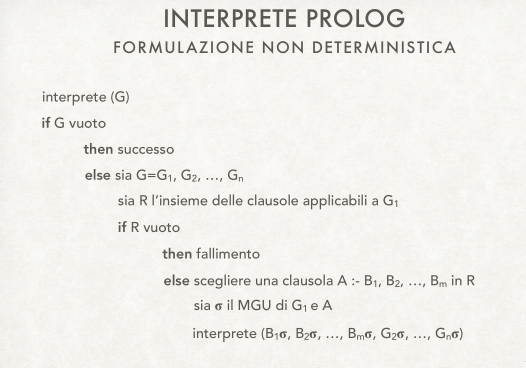
\includegraphics[scale=0.4]{02/Interprete PROLOG.png}
    \caption{Una formulazione non deterministica di come funziona l'interprete PROLOG.}
\end{figure}

\nt{MGU è il Most General Unifier: minimo sforzo per rendere uguali due variabili (il fatto e il goal).}

\begin{itemize}
  \item La computazione ha successo se esiste una computazione che
termina con successo. 
\item Non determinismo: non è specificata la regola scelta in R. 
\item Ma l'interprete PROLOG si comporta in modo \fancyglitter{deterministico}: 
  \begin{itemize}
    \item Le clausole vengono considerate nell’ordine in cui sono scritte
nel programma. 
\item Viene fatto backtracking all’ultimo punto di scelta ogni volta
che la computazione fallisce.
  \end{itemize}
\item In caso di successo, l’interprete restituisce una sostituzione per le
variabili che compaiono nel goal.
\end{itemize}

\subsection{Breve Ripasso di Logica}

\dfn{Logica Classica}{
Conseguenza logica definita semanticamente: dato una teoria e una formula, diciamo che la formula segue dalla
teoria se essa è vera in tutti i modelli della teoria.
}

\ex{Gatti}{
  \begin{itemize}
    \item I gatti miagolano: gatto $\rightarrow$ miagola. 
    \item I persiani sono gatti: persiano $\rightarrow$ gatto.
    \item Si vuole dimostrare che i persiani miagolano: k $\vDash$ persiano $\rightarrow$ miagola.
  \end{itemize} 
  \begin{center}
    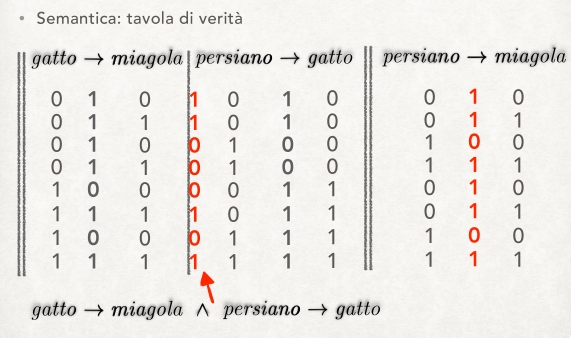
\includegraphics[scale = 0.4]{02/gatto.png}
  \end{center}
}

\begin{itemize}
  \item Tuttavia il processo è molto laborioso già con poche formule e basi di conoscenza piccole. 
  \item Metodo di prova: procedura/algoritmo che calcola/dimostra se una formula è
conseguenza logica della teoria. 
\begin{itemize}
  \item \fancyglitter{Corretto}: se l’algoritmo dimostra F da K, allora F è
conseguenza logica di K. 
\item \fancyglitter{Completo}: se F è conseguenza logica di K, allora l’algoritmo
dimostra F da K.
\end{itemize}
\end{itemize}

\paragraph{Risoluzione:}

\begin{itemize}
  \item Si applica a formule in forma di \fancyglitter{clausole} (disgiunzioni di letterali\footnote{Formule atomiche o negazione di formule atomiche.}). 
  \item Si basa su un'unica regola di inferenza: 
    \begin{itemize}
      \item Date due clausole $C_1=A_1 \lor \dots \lor A_n$ e $C_2=B_1 \lor \dots \lor B_m$. 
      \item Se ci sono due letterali $A_i$ e $B_j$ tali che $A_i = \neg B_j$, allora posso derivare la clausola \fancyglitter{risolvente} $A_1 \lor \dots A_{i-1} \lor A_{i+1} \lor \dots \lor A_n \lor B_1 \lor \dots B_{j-1} \lor B_{j+1} \lor \dots \lor B_m$. 
      \item Il risolvente è conseguenza logica di $C_1 \cup C_2$
    \end{itemize}
  \item Data una teoria (insieme di formule) $K$ e una formula $F$, dimostro
che $F$ è conseguenza logica di $K$ per refutazione (dimostrare che $K \cup \neg F$ è inconsistente). 
\item Si parte dalle clausole $K \cup \neg F$, risolvendo a ogni passo due
clausole e aggiungendo il risolvente all’insieme di clausole. 
\item Si conclude quando si ottiene la clausola vuota.
\end{itemize}

\ex{Risoluzione gatti}{
  \begin{center}
    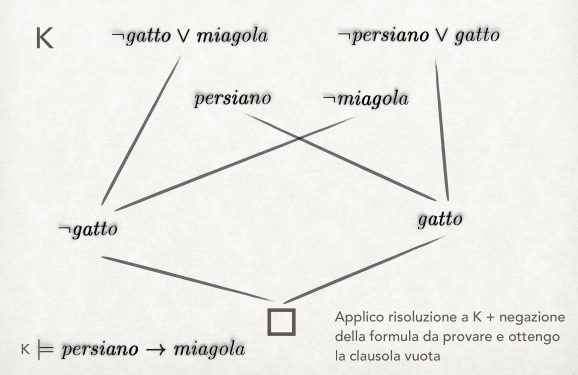
\includegraphics[scale=0.5]{02/ris.png}
  \end{center}
}

\paragraph{Inoltre:}

\begin{itemize}
  \item Se le due clausole $C_1=A_1 \lor \dots \lor A_n$ e $C_2=B_1 \lor \dots \lor B_m$ contengono variabili, i due letterali $A_i$ e $B_j$ devono essere tali che si possa fare l’\fancyglitter{unificazione} tra i due: 
    \begin{itemize}
      \item Unificazione: sostituzione $\alpha$ di variabili con termini o uguaglianza di variabili affinché $A_i=\neg B_j$.
      \item Clausola risolvente $[A_1 \lor \dots A_{i-1} \lor A_{i+1} \lor \dots \lor A_n \lor B_1 \lor \dots B_{j-1} \lor B_{j+1} \lor \dots \lor B_m] \alpha$. 
      \item Le sostituzioni di $\alpha$ sono applicate a $A_1 \lor \dots A_{i-1} \lor A_{i+1} \lor \dots \lor A_n \lor B_1 \lor \dots B_{j-1} \lor B_{j+1} \lor \dots \lor B_m$.
    \end{itemize}
\end{itemize}

\begin{figure}[h]
    \centering
    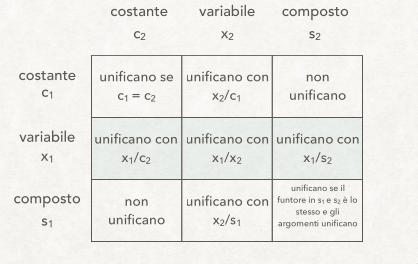
\includegraphics[scale=0.7]{02/uni.png}
    \caption{Unificazione di due termini.}
\end{figure}

\nt{Per ragioni d'efficienza, PROLOG non fa \fancyglitter{occur check}, ossia una variabile X unifica con f(X).}

\subsection{Risoluzione SLD}

Per arrivare a un linguaggio di programmazione PROLOG si vuole una strategia efficiente. 

\dfn{Risoluzione SLD}{
  Linear resolution with Selection function for Definite clauses: 
  \begin{itemize}
    \item K con clausole \newfancyglitter{definite}:
      \begin{itemize}
        \item Clausole di Horn: al più un letterale non negato. 
        \item Strategia linear input: a ogni passo di risoluzione, una \newfancyglitter{variante} di
una clausola è sempre scelta nella K di partenza (programma)
mentre l’altra è sempre il risolvente del passo precedente (goal, la
negazione di F al primo passo). 
\item Variante: clausola con variabili rinominate.
      \end{itemize}
  \end{itemize}
}

\nt{\underline{\textbf{\textit{NON}}} LSD.}

\qs{}{Ma perché ci si limita alle clausole di Horn?}

\paragraph{Risposta:} si rimuove la parte "intuitiva" che non può essere implementata nel PROLOG. Inoltre le clausole di Horn garantiscono la completezza.

\paragraph{Derivazione SLD per un goal $G_0$ da un insieme di clausole K è:}

\begin{itemize}
  \item Una sequenza di clausole goal $G_0, G_1, \dots, G_n$. 
  \item Una sequenza di varianti di clausole di $K C_1, C_2, \dots, C_n$. 
  \item Una sequenza di MGU $\alpha_1, \alpha_2, \dots, \alpha_n$, tali che $G_{i+1}$ è derivato da $G_i$ e da $C_{i+1}$
    attraverso la sostituzione $\alpha_{i+1}$,
\end{itemize}

\paragraph{Tre possibili tipi di derivazioni:}

\begin{itemize}
  \item Successo se $G_n$ è vuoto (\texttt{true}). 
  \item Fallimento finito, se non è possibile derivare da $G_n$ alcun risolvente e $G_n$ non è vuoto (\texttt{false}).
  \item Fallimento infinito, se è sempre possibile derivare nuovi risolventi (loop infinito).
\end{itemize}

\paragraph{Due forme di non determinismo:}

\begin{itemize}
  \item Regola di calcolo per selezionare a ogni passo l’atomo $B_i$
del goal da unificare con una clausola. 
\item Scelta di quale clausola utilizzare a ogni passo di
risoluzione. 
\end{itemize}

\dfn{Regola di calcolo}{
Funzione che ha come dominio l’insieme dei
goal e per ogni goal seleziona un suo atomo.
}

\nt{La regola di calcolo non influenza correttezza e completezza del metodo di prova.}

\qs{}{Come si costruisce l'albero SLD?}

\paragraph{Data una regola di calcolo, è possibile rappresentare tutte le
derivazioni con un albero SLD:}

\begin{itemize}
  \item Nodo: goal. 
  \item Radice: goal iniziale $G_0$. 
  \item Ogni nodo $\leftarrow A_1, \dots, A_m, \dots, A_k$, dove $A_m$ è l’atomo
selezionato dalla regola di calcolo, ha un figlio per ogni
clausola A $\leftarrow B_1, \dots, B_k$ tale che $A$ e $A_m$ sono unificabili con
MGU $\alpha$. Il nodo figlio è etichettato con il goal $\leftarrow [A_1, \dots, A_{m-1}, B_1, \dots, B_k, A_{m+1}, \dots, A_k] \alpha$. Il ramo dal padre al figlio è
etichettato con $\alpha$ e con la clausola selezionata.
\end{itemize}

\paragraph{Scelte per rendere la strategia deterministica:}

\begin{itemize}
  \item Regola di computazione: \fancyglitter{leftmost} (viene sempre scelto il sottogoal più a sinistra). 
  \item Clausole considerate nell’\fancyglitter{ordine in cui sono scritte nel programma}. 
  \item Strategia di ricerca: \fancyglitter{in profondità con backtracking}. 
    \begin{itemize}
      \item Non è completa perché se una computazione che porta al successo si trova a destra di un ramo infinito l'interprete non la trova, perché entra, senza mai uscirne, nel ramo infinito.
    \end{itemize}
\end{itemize}

\nt{Cercare di mettere a destra le computazioni che possano produrre eventuali casini.}

\subsection{Il Cut}

\dfn{Cut}{
  Il \newfancyglitter{cut} è un predicato extra-logico che consente di modificare l'esecuzione dell'interprete PROLOG. CUT (!): 
  \begin{itemize}
    \item Predicato sempre vero. 
    \item Se eseguito blocca il backtracking.
  \end{itemize}
}

\nt{Si rischia di perdere la completezza, ma si guadagna molto in efficienza.}

\paragraph{Modello run-time dell'interprete PROLOG:}

\begin{itemize}
  \item Due stack: 
    \begin{itemize}
      \item Stack di \fancyglitter{esecuzione}: contiene i record di
attivazione (environment) dei predicati in
esecuzione. 
\item Stack di \fancyglitter{backtracking}: contiene l'insieme dei punti di scelta (choice-point).
    \end{itemize}
  \item In realtà c'è un solo stack, con alternanza di environment e choice-point.
\end{itemize}

\paragraph{Il cut:}

\begin{itemize}
  \item Rende definitive le scelte fatte nel corso della valutazione dall'interprete PROLOG (eliminazione di choice-point dallo stack di backtracking). 
  \item Altera il controllo del programma. 
  \item Perdità di dichiaratività.
\end{itemize}

\begin{figure}[h]
    \centering
    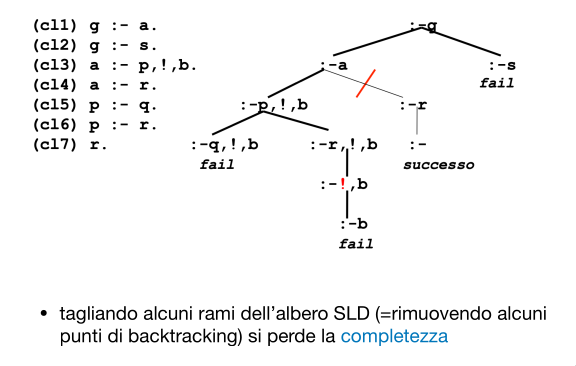
\includegraphics[scale=0.7]{02/cut.png}
    \caption{Esempio di cut che provoca la perdita di completezza.}
\end{figure}

\section{Strategie di Ricerca in PROLOG}

\paragraph{Un problema di ricerca è definito da:} 
    \begin{itemize}
    \item \fancyglitter{Stato iniziale}. 
    \item \fancyglitter{Insieme delle azioni} (azione: fa passare da uno stato all'altro). 
    \item Specifica degli obiettivi (goal).
    \item Costo di ogni azione.
    \end{itemize}

\nt{Non tutti i problemi hanno una naturale soluzione con la ricerca nello spazio degli stati.}



\subsection{Ricerca nello Spazio degli Stati}

\dfn{Soluzione a un Problema}{

}

\cor{Soluzione Ottima}{

}
















